% Handout «Der Stromkrieg» – Modul «Weltmacht USA» (FHNW), Simon Bruder
% Kompilieren mit pdfLaTeX und Biber (Overleaf erkennt beides automatisch).
%
% Quellen nach IEEE, wie es die FHNW empfiehlt (Seitenzahl im Verweis, Punkt nach der Klammer):
%   \cite{edpCW}          ergibt [1]           Online-Quelle ohne Seitenzahl
%   \cite[994]{kaick}     ergibt [3, S. 994]   Buch oder Artikel mit Seitenzahl
%   \citeoffen{jonnes}    ergibt [9, S. ?]     Seitenzahl fehlt noch (rot markiert)
% Hast du eine Seitenzahl nachgeschlagen, ersetzt du \citeoffen{...} durch \cite[Seite]{...}.

\documentclass[10pt,a4paper]{article}
% Einstellungen für das Handout: Layout, Farben, Bausteine und Quellen nach IEEE (deutsch, FHNW-Leitfaden).
% Hier musst du normalerweise nichts ändern. Der Text steht in main.tex, die Quellen in quellen.bib.

\usepackage[T1]{fontenc}
\usepackage[utf8]{inputenc}
\usepackage[nswissgerman]{babel}
\usepackage[autostyle,german=swiss]{csquotes}
\usepackage[default]{sourcesanspro}   % dieselbe Schrift wie auf den Folien (Source Sans)
\usepackage{microtype}
\usepackage[a4paper,left=18mm,right=18mm,top=27mm,bottom=19mm,
            headheight=11mm,headsep=7mm,footskip=9mm]{geometry}
\usepackage{graphicx}
\usepackage{xcolor}
\usepackage{fancyhdr}
\usepackage{titlesec}
\usepackage{enumitem}
\usepackage{tabularx,booktabs,array}
\usepackage{caption}
\usepackage{multicol}
\usepackage[most]{tcolorbox}
\usepackage{fontawesome5}
\usepackage{qrcode}
\usepackage{pgfplots}
\pgfplotsset{compat=1.17}
\usepackage[backend=biber,style=ieee,sorting=none,dashed=false,urldate=long]{biblatex}
\addbibresource{quellen.bib}
\usepackage[hidelinks]{hyperref}

% ---------- Farben: eine Hauptfarbe (Marineblau) und eine Akzentfarbe (Kupfer), wie auf den Folien ----------
% Kupfer steht durchgehend für Gleichstrom und Edison, Marineblau für Wechselstrom und Westinghouse.
\definecolor{navy}{HTML}{10233F}
\definecolor{kupfer}{HTML}{C8641E}
\definecolor{grau}{HTML}{5F6B7A}
\definecolor{hell}{HTML}{EEF1F5}
\definecolor{kupferhell}{HTML}{FBF1E9}
\AtBeginDocument{\color{navy}}

% ---------- Verweise mit noch fehlender Seitenzahl ----------
% \citeoffen{jonnes} ergibt im Entwurf [1, S. ?] in Rot, in der Endfassung [1].
\newif\ifentwurf
\entwurftrue
\newcommand{\citeoffen}[1]{\ifentwurf\cite[{\color{red}S.\,?}]{#1}\else\cite{#1}\fi}
\newcommand{\offen}[1]{\ifentwurf\textcolor{red}{[#1]}\fi}   % sonstige offene Stellen, nur im Entwurf sichtbar

% ---------- Quellenverzeichnis: IEEE mit deutschen Angaben wie im FHNW-Leitfaden ----------
\stdpunctuation                                                    % «Titel», Zeitschrift (Komma nach dem Schlusszeichen)
\DefineBibliographyStrings{nswissgerman}{jourvol = {Bd\adddot}}   % Bd. statt Jg.
\DeclareFieldFormat{url}{\mkbibbrackets{Online}\adddot\space Verfügbar unter\addcolon\space\url{#1}}
\DeclareFieldFormat{urldate}{\mkbibbrackets{Zugegriffen\addcolon\space#1}}
\renewcommand*{\bibfont}{\footnotesize\raggedright}
\setlength{\bibitemsep}{1.5pt}
% Webseiten: Urheber, «Titel», Organisation, Datum. [Online]. Verfügbar unter: Adresse [Zugegriffen: Datum].
\DeclareBibliographyDriver{online}{%
  \usebibmacro{bibindex}%
  \usebibmacro{begentry}%
  \usebibmacro{author/editor+others/translator+others}%
  \setunit{\labelnamepunct}\newblock
  \usebibmacro{title}%
  \newunit\newblock
  \printlist{organization}%
  \newunit\newblock
  \usebibmacro{date}%
  \setunit{\adddot\addspace}\newblock
  \usebibmacro{url+urldate}%
  \usebibmacro{finentry}}

% ---------- Seitenlayout ----------
\pagestyle{fancy}
\fancyhf{}
\fancyhead[L]{
\includegraphics[height=9mm]{bilder/fhnw_logo.jpg}}
\fancyhead[R]{\footnotesize\color{grau}Modul «Weltmacht USA» \textperiodcentered{} Handout}
\fancyfoot[L]{\footnotesize\color{grau}FHNW, School of Engineering, Windisch \textperiodcentered{} Dozent: Stephan Schwarz}
\fancyfoot[R]{\footnotesize\color{grau}\thepage}
\renewcommand{\headrulewidth}{0.4pt}
\renewcommand{\footrulewidth}{0pt}
\renewcommand{\headrule}{{\color{navy!30}\hrule width\headwidth height\headrulewidth}}

\setlength{\parindent}{0pt}
\setlength{\emergencystretch}{1.5em}
\setlength{\parskip}{4pt plus 1pt}
\setcounter{secnumdepth}{0}
% Überschriften mit kurzem Kupferstrich
\titleformat{\section}{\large\bfseries\color{navy}}{}{0pt}{}[{\vspace{-3pt}\textcolor{kupfer}{\rule{11mm}{1.3pt}}}]
\titlespacing*{\section}{0pt}{11pt plus 2pt minus 2pt}{3pt}
\setlist{nosep,leftmargin=*}
\renewcommand{\arraystretch}{1.25}
\newcolumntype{L}[1]{>{\raggedright\arraybackslash}p{#1}}
\newcolumntype{Y}{>{\raggedright\arraybackslash}X}
\captionsetup{labelsep=colon,skip=4pt,font={footnotesize,color=grau},labelfont={bf,color=navy},justification=raggedright,singlelinecheck=false}
\captionsetup[table]{name=Tab.,position=bottom}
\captionsetup[figure]{name=Abb.}

% ---------- Bausteine ----------
% Leitfrage (dunkel) und Kurzantwort (hell)
\newtcolorbox{leitfrage}{enhanced,colback=navy,colframe=navy,coltext=white,arc=1.5mm,boxrule=0pt,
  left=4mm,right=4mm,top=2.6mm,bottom=2.6mm,fontupper=\normalsize,
  colbacklower=hell,collower=navy,fontlower=\normalsize,lowerbox=visible,segmentation style={draw=none},
  bicolor,boxsep=0pt,middle=2.6mm}
\newcommand{\etikett}[1]{{\footnotesize\bfseries\color{kupfer}\MakeUppercase{#1}}\par\vspace{1pt}}
% Karte mit farbigem Balken oben: \begin{karte}{Farbe}{Titel} ... \end{karte}
\newtcolorbox{karte}[2]{enhanced,colback=white,colframe=#1,boxrule=0.4pt,toprule=2.2pt,arc=1.2mm,
  left=3mm,right=3mm,top=2mm,bottom=2mm,boxsep=0pt,
  title={#2},fonttitle=\bfseries,coltitle=navy,attach title to upper={\par\vspace{2pt}}}
% Kachel mit grosser Zahl: \kennzahl{Farbe}{Zahl}{Erklärung}
\newcommand{\kennzahl}[3]{\begin{tcolorbox}[enhanced,colback=hell,colframe=hell,arc=1.2mm,boxrule=0pt,
  left=3mm,right=3mm,top=2mm,bottom=2mm,boxsep=0pt]
  {\fontsize{24}{26}\selectfont\bfseries\color{#1}#2}\par\vspace{1pt}{\footnotesize\raggedright #3\par}\end{tcolorbox}}
% Nummerierter Punkt: \punkt{1}{Titel}{Text}
\newcommand{\punkt}[3]{\begin{tcolorbox}[enhanced,colback=white,colframe=navy!18,boxrule=0.4pt,arc=1.2mm,
  left=3mm,right=3mm,top=2mm,bottom=2mm,boxsep=0pt]
  {\fontsize{20}{20}\selectfont\bfseries\color{kupfer}#1}\hspace{2mm}{\bfseries #2}\par\vspace{2pt}{\small\raggedright #3\par}\end{tcolorbox}}
% Zeile mit Symbol: \symbolzeile{\faBolt}{Titel}{Text}
\newcommand{\symbolzeile}[3]{\par\noindent\begin{minipage}[t]{6mm}\centering\color{kupfer}#1\end{minipage}%
  \begin{minipage}[t]{\dimexpr\linewidth-6mm}\raggedright\textbf{#2} #3\end{minipage}\par\vspace{3pt}}
% QR-Code mit Beschriftung: \qr{Adresse}{Titel}{Beschreibung}
\newcommand{\qr}[3]{\begin{minipage}[t]{15mm}\vspace{0pt}\qrcode[height=14mm]{#1}\end{minipage}\hspace{2.5mm}%
  \begin{minipage}[t]{\dimexpr\linewidth-17.5mm}\vspace{0pt}\raggedright\small\textbf{#2}\par #3\end{minipage}}

% Ereignis auf dem Zeitstrahl: \ereignis{Jahr}{oben|unten}{Titel}{Text}; 1882 liegt bei x = 15 mm, ein Jahr = 10,286 mm
\newcommand{\zeitx}[1]{15+(#1-1882)*10.286}
\newcommand{\ereignis}[4]{%
  \ifstrequal{#2}{oben}
    {\draw[navy!35,line width=0.5pt] ({\zeitx{#1}},1.4) -- ++(0,3.6);
     \node[anchor=south,align=center,text width=29mm,inner sep=0.8pt,font=\footnotesize]
       at ({\zeitx{#1}},5.2) {{\bfseries\color{kupfer}#1}\\[-1.5pt]\textbf{#3}\\[-1.5pt]{\scriptsize\color{grau}#4}};}
    {\draw[navy!35,line width=0.5pt] ({\zeitx{#1}},-1.4) -- ++(0,-3.6);
     \node[anchor=north,align=center,text width=29mm,inner sep=0.8pt,font=\footnotesize]
       at ({\zeitx{#1}},-5.2) {{\bfseries\color{kupfer}#1}\\[-1.5pt]\textbf{#3}\\[-1.5pt]{\scriptsize\color{grau}#4}};}
  \fill[white] ({\zeitx{#1}},0) circle (1.9);
  \fill[navy] ({\zeitx{#1}},0) circle (1.25);}
% Begriff im Glossar
\newcommand{\begriff}[2]{\par\noindent\textbf{#1}\quad #2\par\vspace{3pt}}

% ---------- Grafiken: Zahlen in der Textschrift ----------
\pgfplotsset{/pgf/number format/assume math mode=true}

\hypersetup{pdftitle={Der Stromkrieg – Handout},pdfauthor={Simon Bruder},pdflang={de-CH}}

% Endfassung: die folgende Zeile aktivieren, dann verschwinden die roten «S. ?».
% \entwurffalse

\begin{document}

\begin{center}
  {\fontsize{18}{22}\selectfont\bfseries Der Stromkrieg -- Handout\par}
  \vspace{1.5mm}
  Edison vs.\ Tesla -- und die Rolle von George Westinghouse\par
  Simon Bruder \textperiodcentered{} Modul «Weltmacht USA» \textperiodcentered{} Dozent: Stephan Schwarz
  \textperiodcentered{} 10.12.2026
\end{center}

\section{Worum geht es?}
\begin{spalte}{0.655\linewidth}
  Elektrisches Licht war in den 1880er-Jahren ein neues Geschäft (Abb.~\ref{abb:karikatur}). Im
  \textbf{«Stromkrieg»} («War of the Currents») stritten die Firmen der Erfinder um das Stromsystem der USA, vor allem
  in den späten 1880er- und frühen 1890er-Jahren \cite{edpCW}. «Edison gegen Tesla» heisst:
  \textbf{Gleichstrom gegen Wechselstrom}.
  \begin{itemize}
    \item \textbf{Thomas Edison} lieferte ab 1882 in New York Gleichstrom. Ein Kraftwerk reichte nur für ein
      Quartier \cite{pearl}.
    \item \textbf{Nikola Tesla} arbeitete 1884 sechs Monate für Edison; dann trennten sie sich \cite[994]{kaick}.
      Noch 1931 kritisierte er Edisons Methode: viel Probieren, wenig Theorie \citeoffen{nyt31}.
    \item \textbf{George Westinghouse} kaufte 1888 Teslas Wechselstrompatente und baute die Netze
      \cite[994]{kaick}.
    \item \textbf{Kampagne:} Edisons Lager warnte vor Wechselstrom. Harold P. Brown tötete öffentlich Tiere und half,
      den elektrischen Stuhl einzuführen \citeoffen{hughes58}.
  \end{itemize}
\end{spalte}\hfill
\begin{spalte}{0.31\linewidth}
  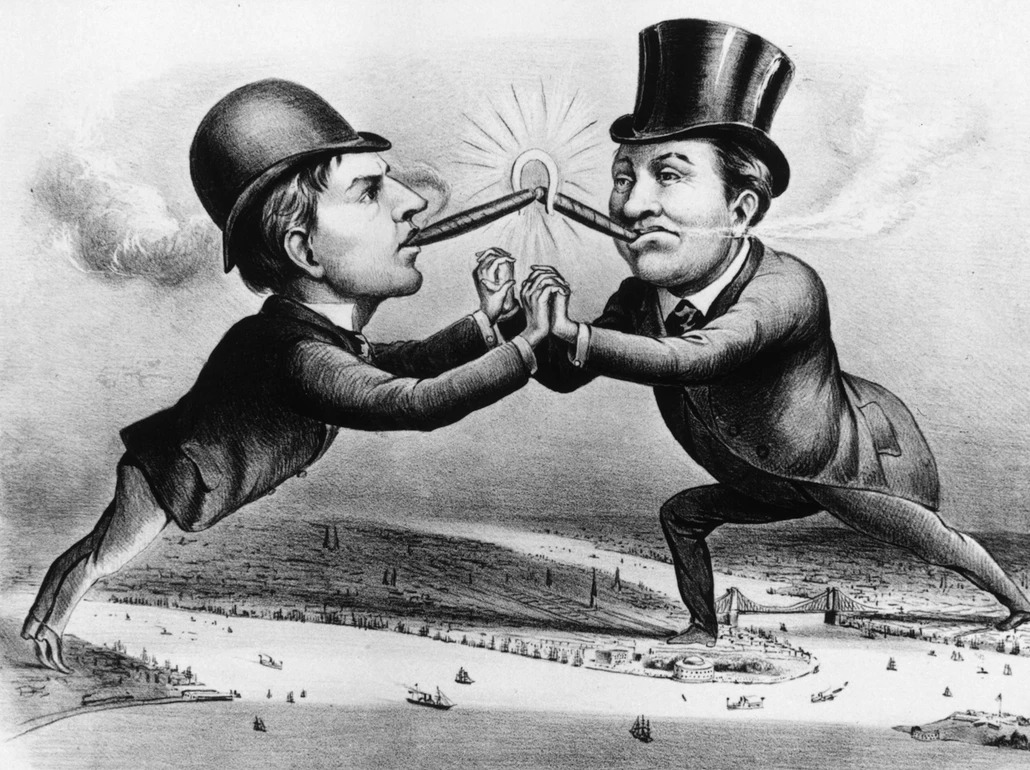
\includegraphics[width=\linewidth]{bilder/karikatur_edison_brush.jpg}
  \captionof{figure}{Edison (links) und Charles Brush, der Erfinder der Bogenlampe, als Rivalen um die Beleuchtung
    New Yorks. Druck von Currier \& Ives, spätes 19.~Jahrhundert. Bild: MPI/Getty Images, aus \cite{natgeo}.}
  \label{abb:karikatur}
\end{spalte}

\vspace{3mm}
\begin{tabularx}{\linewidth}{|Y|}
  \hline
  \textbf{Leitfrage:} Warum setzte sich Teslas Wechselstrom gegen Edisons Gleichstrom durch -- und was zeigt der
  Konflikt über den Aufstieg der USA zur führenden Industriemacht? \\ \hline
  \textbf{These:} Nicht der berühmtere Erfinder gewann, sondern das billigere System mit dem stärkeren Geldgeber.
  Aus dem Streit gingen Grosskonzerne hervor, typisch für den amerikanischen Industriekapitalismus. \\ \hline
\end{tabularx}

\begin{tabelle}{Zwei Systeme um 1888: Stärken und Schwächen}
\begin{tabularx}{\linewidth}{|C{21mm}|Y|Y|}
  \hline
  & \kopf{Gleichstrom -- Edison} & \kopf{Wechselstrom -- Tesla und Westinghouse} \\ \hline
  Stärken & niedrige Spannung (rund 110\,V), gilt als sicherer; Akkus speichern Strom; erprobte Motoren &
    Transformator: hohe Spannung, wenig Verlust, weite Strecken; wenige grosse Kraftwerke, auch Wasserkraft
    \cite[994]{kaick} \\ \hline
  Schwächen & hohe Leitungsverluste: ein Kraftwerk pro Quartier, viel Kupfer \cite{pearl} & Hochspannung ist
    lebensgefährlich: 1889 starb in Manhattan ein Arbeiter in den Leitungen \citeoffen{essig} \\ \hline
  Argument & Sicherheit: 1889 schrieb Edison, nichts rechtfertige Hochspannung und Wechselstrom
    \citeoffen{edison89} & Kosten: billiger Strom über weite Strecken, z.\,B. von den Niagarafällen nach Buffalo
    \citeoffen{jonnes} \\ \hline
  Geldgeber & Bankier J.\,P. Morgan \citeoffen{jonnes} & George Westinghouse \cite[994]{kaick} \\ \hline
\end{tabularx}
\end{tabelle}

\par\addvspace{6pt}
\begin{spalte}{0.805\linewidth}
\captionof{table}{Die wichtigsten Etappen}
\small
\begin{tabularx}{\linewidth}{|C{9mm}|Y|}
  \hline
  \textbf{Jahr} & \kopf{Ereignis} \\ \hline
  1882 & Edison eröffnet in New York sein erstes Kraftwerk (Pearl Street): Gleichstrom für rund 85 Kunden und
    400 Lampen \cite{pearl}. \\ \hline
  1884 & Tesla, Ingenieur aus Smiljan (heute Kroatien), arbeitet in New York für Edison. Nach sechs Monaten
    trennen sie sich \cite[993--994]{kaick}. \\ \hline
  1888 & Westinghouse kauft im Juli Teslas Wechselstrompatente \cite[994]{kaick}. Edisons Lager startet die
    Kampagne: Harold P. Brown tötet öffentlich Hunde \citeoffen{hughes58}. \\ \hline
  1890 & Erste Hinrichtung auf dem elektrischen Stuhl (Abb.~\ref{abb:stuhl}) \citeoffen{essig}. Den Generator von
    Westinghouse hatte Brown gegen dessen Willen beschafft \citeoffen{hughes58}. \\ \hline
  1891 & Westinghouse gerät in Finanznot; Tesla verzichtet auf seine Lizenzgebühren \citeoffen{carlson}. \\ \hline
  1892 & Edisons Firma fusioniert mit Thomson-Houston zu General Electric, eingefädelt von Banken um J.\,P. Morgan.
    Edisons Name verschwindet \citeoffen{jonnes}. \\ \hline
  1893 & Westinghouse versorgt die Weltausstellung in Chicago mit Teslas Wechselstromsystem \cite[994]{kaick}. \\
    \hline
  1896 & Strom von den Niagarafällen fliesst rund 40\,km nach Buffalo \citeoffen{jonnes}, mit Teslas System
    \cite[994]{kaick}. \\ \hline
\end{tabularx}
\end{spalte}\hfill
\begin{spalte}{0.17\linewidth}
  \vspace{5.5mm}
  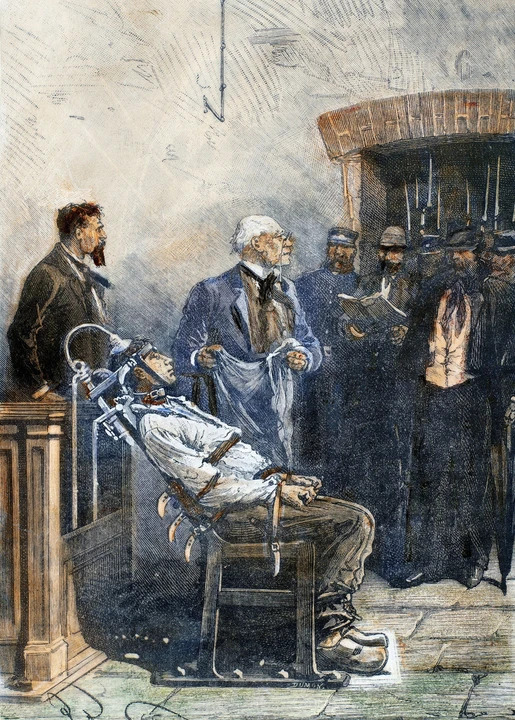
\includegraphics[width=\linewidth]{bilder/elektrischer_stuhl_1890.jpg}
  \captionof{figure}{Erste Hinrichtung auf dem elektrischen Stuhl, 1890. Kolorierte Illustration. Bild:
    Granger/Cordon Press, aus \cite{natgeo}.}
  \label{abb:stuhl}
\end{spalte}

\newpage

\section{Warum gewann Teslas Wechselstrom?}
\begin{itemize}
  \item \textbf{Kosten:} Mit dem Transformator kam Strom mit wenig Verlust über weite Strecken, und wenige grosse
    Kraftwerke reichten; Gleichstrom brauchte viele kleine \citeoffen{jonnes}.
  \item \textbf{Kapital:} Westinghouse brachte Teslas System in die Praxis \cite[994]{kaick}. 1892 ging Edisons Firma
    in General Electric auf, und auch GE setzte auf Wechselstrom \citeoffen{jonnes}.
  \item \textbf{Die Kampagne verpuffte:} Westinghouse ignorierte sie zuerst, bestritt dann die Vorwürfe und machte sie
    schliesslich mit besserer Technik gegenstandslos \citeoffen{cole}.
\end{itemize}

\section{USA und Europa}
\begin{itemize}
  \item \textbf{Gilded Age:} Der Staat regelte kaum. Bankiers wie J.\,P. Morgan finanzierten die Firmen, und die
    Konkurrenten stritten vor Gericht um Patente \citeoffen{jonnes}.
  \item \textbf{Ideen aus Europa:} Den Transformator entwickelten Gaulard und Gibbs; Westinghouse kaufte die US-Rechte
    \citeoffen{jonnes}. Das Drehfeld fand Galileo Ferraris in Turin zur selben Zeit wie Tesla \citeoffen{carlson}. 1891
    übertrugen die Maschinenfabrik Oerlikon und die AEG Drehstrom über 175\,km von Lauffen nach Frankfurt \cite{steig}.
  \item \textbf{Zwei Normen bis heute:} USA 120\,V und 60\,Hz, Schweiz 230\,V und 50\,Hz \cite{iec}. Standards aus
    der Pionierzeit bleiben lange bestehen (Pfadabhängigkeit) \citeoffen{david92}.
\end{itemize}

\section{Bedeutung für die Weltmacht USA}
\begin{spalte}{0.50\linewidth}
\begin{itemize}
  \item \textbf{Industriemacht:} Zwischen 1880 und 1900 überholten die USA Grossbritannien als grösste
    Industriemacht (Abb.~\ref{abb:weltindustrie}) \citeoffen{bairoch}.
  \item \textbf{Billiger Strom für die Fabriken:} Elektromotoren lieferten 1899 knapp 5\,\%, 1929 rund 78\,\% der
    Antriebsleistung der US-Industrie \citeoffen{devine}.
  \item \textbf{Grosskonzerne:} General Electric und Westinghouse teilten ab 1896 ihre Patente und beherrschten den
    Markt \citeoffen{jonnes}.
\end{itemize}
\end{spalte}\hfill
\begin{spalte}{0.47\linewidth}
  \vspace{-2mm}
  \begin{tikzpicture}
    \begin{axis}[
        width=0.70\linewidth, height=34mm,
        xmin=1856, xmax=1915, ymin=0, ymax=36,
        xtick={1860,1880,1900,1913},
        x tick label style={/pgf/number format/1000 sep={}},
        ytick={0,10,20,30}, yticklabel={\pgfmathprintnumber{\tick}\,\%},
        axis lines=left, axis line style={-}, tick align=outside,
        ymajorgrids, grid style={black!12},
        tick label style={font=\footnotesize},
        clip=false,
      ]
      % Zeitraum des Stromkriegs
      \addplot[draw=none, fill=black!10, forget plot] coordinates {(1886,0) (1886,36) (1892,36) (1892,0)} \closedcycle;
      \node[font=\scriptsize\itshape, anchor=south] at (axis cs:1889,36) {Stromkrieg};
      % Werte nach Bairoch: Stichjahre 1860, 1880, 1900, 1913
      \addplot[usa, line width=1.4pt, mark=*, mark size=1.8pt]
        coordinates {(1860,7.2) (1880,14.7) (1900,23.6) (1913,32.0)}
        node[right=2pt, black, font=\footnotesize] {\textbf{32,0\,\%} USA};
      \addplot[grossbritannien, line width=1.2pt, dashed, mark=square*, mark size=1.6pt, mark options={solid}]
        coordinates {(1860,19.9) (1880,22.9) (1900,18.5) (1913,13.6)}
        node[right=2pt, yshift=-4pt, black, font=\footnotesize] {\textbf{13,6\,\%} Grossbritannien};
      \addplot[deutschland, line width=1.2pt, densely dotted, mark=triangle*, mark size=2pt, mark options={solid}]
        coordinates {(1860,4.9) (1880,8.5) (1900,13.2) (1913,14.8)}
        node[right=2pt, yshift=4pt, black, font=\footnotesize] {\textbf{14,8\,\%} Deutschland};
    \end{axis}
  \end{tikzpicture}
  \captionof{figure}{Anteil an der Weltindustrieproduktion in Prozent, Stichjahre 1860 bis 1913 (Schätzwerte).
    Eigene Darstellung, Zahlen aus \citeoffen{bairoch}.}
  \label{abb:weltindustrie}
\end{spalte}

\begin{tabelle}{Drei Mythen}
\begin{tabularx}{\linewidth}{|Y|Y|}
  \hline
  \multicolumn{1}{|c|}{\textbf{Mythos}} & \kopf{Befund} \\ \hline
  Edison zeigte öffentlich «grausame Experimente mit Hunden, Pferden und sogar einem Elefanten» \cite{abb}. &
    Die Tierversuche machte Harold P. Brown, mit Hilfe aus Edisons Labor \citeoffen{hughes58}. Topsy starb erst
    1903, ohne Edison \cite{topsy}. \\ \hline
  Edison prellte Tesla um 50'000 Dollar. &
    In Teslas eigenem Bericht von 1919 machte «der Manager» das Versprechen, nicht Edison \citeoffen{tesla19}. \\
    \hline
  Tesla erfand den Wechselstrom allein. &
    Den Transformator gab es schon in Europa \citeoffen{jonnes}; das Drehfeld fand Ferraris gleichzeitig
    \citeoffen{carlson}. \\ \hline
\end{tabularx}
\end{tabelle}

\section{Und heute?}
\begin{itemize}
  \item \textbf{Teslas Wechselstrom} kommt aus jeder Steckdose \cite{iec}.
  \item \textbf{Gleichstrom kehrt zurück:} Akkus, Solaranlagen und E-Autos nutzen Gleichstrom, lange Leitungen die
    Hochspannungs-Gleichstrom-Übertragung (HGÜ, seit 1954) \cite{gotland}. Ab Ende 2028 soll SuedLink Windstrom über
    rund 700\,km nach Süddeutschland bringen \cite{bnetza}.
  \item \textbf{Tesla als Name:} Einheit der magnetischen Flussdichte seit 1960 \cite[994]{kaick}; Autohersteller
    seit 2003 \cite[993]{kaick}, dessen Ladestecker in den USA zur Norm SAE~J3400 wird \cite{nacs}.
  \item \textbf{Edisons Gleichstrom:} In Manhattan schaltete Con Edison den letzten Gleichstromanschluss erst 2007
    ab, 125 Jahre nach Pearl Street \cite{lee}.
\end{itemize}

\section{Fazit}
\begin{itemize}
  \item Teslas Wechselstrom gewann, weil er billiger war: hohe Spannung, wenige grosse Kraftwerke, weite Strecken.
  \item Edisons Sicherheitsbedenken waren nicht erfunden, aber Kosten und Kapital entschieden.
  \item Billiger Strom und Grosskonzerne trugen den Aufstieg der USA zur grössten Industriemacht.
\end{itemize}

\newpage

\section{Glossar}
{\small
\begin{tabularx}{\linewidth}{|C{31mm}|Y|}
  \hline
  Gleichstrom (DC) & «Direct Current»: Strom, der immer in dieselbe Richtung fliesst, z.\,B. aus einer Batterie. \\
    \hline
  Wechselstrom (AC) & «Alternating Current»: Strom, der periodisch die Richtung wechselt; so kommt er aus der
    Steckdose (Europa 50\,Hz, USA 60\,Hz) \cite{iec}. \\ \hline
  Transformator & Setzt die Spannung von Wechselstrom herauf oder herab. Höhere Spannung bedeutet bei gleicher
    Leistung kleineren Strom und kleinere Leitungsverluste ($P_\mathrm{V} = I^2 \cdot R$). \\ \hline
  Drehfeldmotor & Wechselstrommotor, den ein rotierendes Magnetfeld antreibt; Grundlage des Induktionsmotors
    \cite[994]{kaick}. \\ \hline
  Westinghouse Electric & Firma von George Westinghouse; baute Wechselstromnetze mit Teslas Patenten
    \cite[994]{kaick}. \\ \hline
  General Electric (GE) & 1892 aus Edison General Electric und Thomson-Houston entstanden, eingefädelt von Banken
    um J.\,P. Morgan \citeoffen{jonnes}. \\ \hline
  Gilded Age & «Vergoldetes Zeitalter» (ca. 1870--1900), benannt nach einem Roman von Mark Twain: an der
    Oberfläche Wachstum und Reichtum, darunter Korruption und soziale Ungleichheit. \\ \hline
  Robber Barons & «Raubritter»: abschätziger Name für mächtige Unternehmer und Bankiers des Gilded Age, etwa
    J.\,P. Morgan. \\ \hline
\end{tabularx}\par}

\section{Tipps}
\textbf{Romane:} «Licht» von Anthony McCarten (Edison und sein Geldgeber J.\,P. Morgan) und «Die letzten Tage der
Nacht» von Graham Moore (Westinghouses Anwalt Paul Cravath); SRF Kultur stellt beide vor \cite{srf}.
\textbf{Film:} «The Current War» (2017). Romane und Film sind Fiktion und keine Quelle.

% Falls das Modul eine Angabe zum Einsatz von KI-Werkzeugen verlangt: die nächste Zeile aktivieren und anpassen.
% {\footnotesize Hinweis: Bei Recherche, Struktur und Formulierung wurde ein KI-Werkzeug eingesetzt; alle Inhalte und Quellen hat der Autor geprüft.\par}

\printbibliography[title=Quellen]

\end{document}
